A top down approach was applied to identify the major components in the system. The client's requirements were the starting point for identifying those components. They were
clear and simple enough to create a high level view of the framework , with which to explain the framework's basic behaviour see figure ~\ref{fig:sprints}. 

\begin{figure}[htp]
\centering
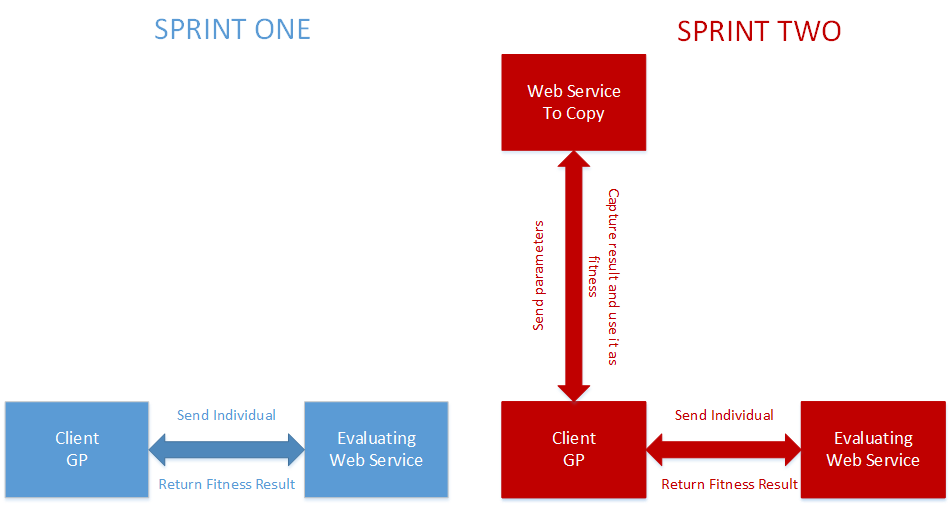
\includegraphics[scale=0.6]{Figures/sprints.png}
\caption{Top level view of sprint one and two. Sprint one is focused on evaluating an individual over the web and sprint two focuses on cloning a web services}
\label{fig:sprints}
\end{figure}

By displaying the way the high level components communicate it was later possible to identify their functionality and split them into lower level components or classes.
This way high cohesion and loose coupling was achieved at every level.
